\begin{figure}[H]
  \centering
  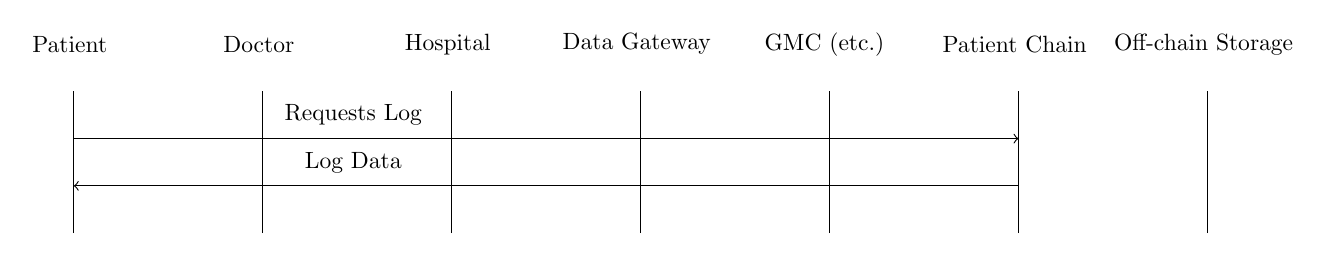
\begin{tikzpicture}[scale = 0.6, every node/.style={scale = 0.85}, every node/.append style={fill = white, rounded corners = 2pt, inner sep = 2pt, align = center} ]

  % Lines
  \draw (4, 17) -- (4, 20);
  \draw (8, 17) -- (8, 20);
  \draw (12, 17) -- (12, 20);
  \draw (16, 17) -- (16, 20);
  \draw (20, 17) -- (20, 20);
  \draw (24, 17) -- (24, 20);
  \draw (28, 17) -- (28, 20);

  % Headings
  \node at (4, 21) { Patient };
  \node at (8, 21) { Doctor };
  \node at (12, 21) { Hospital };
  \node at (16, 21) { Data Gateway };
  \node at (20, 21) { GMC (etc.) };
  \node at (24, 21) { Patient Chain };
  \node at (28, 21) { Off-chain Storage };

  % Arrows
  \node at (10, 19.5) { Requests Log };
  \draw [ -> ] (4, 19) -- (24, 19);

  \node at (10, 18.5) { Log Data };
  \draw [ -> ] (24, 18) -- (4, 18);

  \end{tikzpicture}
  \caption{
    Patient retrieves log of accesses to their account without logging their access
  }
  \label{fig:user_story_04b}
\end{figure}
